%%%%%%%%%%%%%%%%%%%%%%%%%%%%%%%%%%%%%%%%%
% Beamer Presentation
% LaTeX Template
% Version 1.0 (10/11/12)
%
% This template has been downloaded from:
% http://www.LaTeXTemplates.com
%
% License:
% CC BY-NC-SA 3.0 (http://creativecommons.org/licenses/by-nc-sa/3.0/)
%
%%%%%%%%%%%%%%%%%%%%%%%%%%%%%%%%%%%%%%%%%

%----------------------------------------------------------------------------------------
%	PACKAGES AND THEMES
%----------------------------------------------------------------------------------------

\documentclass[usenames,dvipsnames]{beamer}

\mode<presentation> {

% The Beamer class comes with a number of default slide themes
% which change the colors and layouts of slides. Below this is a list
% of all the themes, uncomment each in turn to see what they look like.

%\usetheme{default}
%\usetheme{AnnArbor}
%\usetheme{Antibes}
%\usetheme{Bergen}
%\usetheme{Berkeley}
%\usetheme{Berlin}
%\usetheme{Boadilla}
\usetheme{CambridgeUS}
%\usetheme{Copenhagen}
%\usetheme{Darmstadt}
%\usetheme{Dresden}
%\usetheme{Frankfurt}
%\usetheme{Goettingen}
%\usetheme{Hannover}
%\usetheme{Ilmenau}
%\usetheme{JuanLesPins}
%\usetheme{Luebeck}
%\usetheme{Madrid}
%\usetheme{Malmoe}
%\usetheme{Marburg}
%\usetheme{Montpellier}
%\usetheme{PaloAlto}
%\usetheme{Pittsburgh}
%\usetheme{Rochester}
%\usetheme{Singapore}
%\usetheme{Szeged}
%\usetheme{Warsaw}

% As well as themes, the Beamer class has a number of color themes
% for any slide theme. Uncomment each of these in turn to see how it
% changes the colors of your current slide theme.

%\usecolortheme{albatross}
%\usecolortheme{beaver}
%\usecolortheme{beetle}
%\usecolortheme{crane}
%\usecolortheme{dolphin}
%\usecolortheme{dove}
%\usecolortheme{fly}
%\usecolortheme{lily}
%\usecolortheme{orchid}
%\usecolortheme{rose}
%\usecolortheme{seagull}
%\usecolortheme{seahorse}
%\usecolortheme{whale}
%\usecolortheme{wolverine}

%\setbeamertemplate{footline} % To remove the footer line in all slides uncomment this line
%\setbeamertemplate{footline}[page number] % To replace the footer line in all slides with a simple slide count uncomment this line

%\setbeamertemplate{navigation symbols}{} % To remove the navigation symbols from the bottom of all slides uncomment this line
}

\usepackage{graphicx} % Allows including images
\graphicspath{ {images/} }
\usepackage{booktabs} % Allows the use of \toprule, \midrule and \bottomrule in tables
\usepackage{minted}
\usepackage{multicol}
\usepackage{appendixnumberbeamer}

\catcode``=\active
\def`#1`{\texttt{#1}}

%----------------------------------------------------------------------------------------
%	TITLE PAGE
%----------------------------------------------------------------------------------------

\title[Tail-call optimization]{Tail-call Optimization in R5} % The short title appears at the bottom of every slide, the full title is only on the title page

\author[Derici \& Scott]{Caner Derici \& Ryan Scott} % Your name
\date{\today} % Date, can be changed to a custom date

\begin{document}

\begin{frame}
\titlepage % Print the title page as the first slide
\end{frame}

%------------------------------------------------

\begin{frame}[fragile]
  \frametitle{Tail Calls}
  The last thing that a program does. \vspace{0.3cm}
\begin{minted}{Scheme}
  (define (fact n i)
    (if (<= n 1) i
        (fact (sub1 n) (* n i))))
\end{minted}

\vspace{0.2cm} as opposed to \vspace{0.2cm}

\begin{minted}{Scheme}
  (define (fact n)
    (if (<= n 1) 1
        (* n (fact (sub1 n)))))
\end{minted}
\end{frame}

\begin{frame}[fragile]
  \frametitle{Tail Calls}
  \begin{center}
    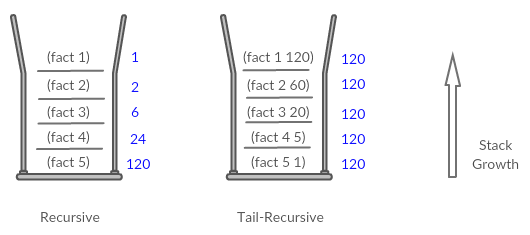
\includegraphics[scale=0.6]{stack.png}
    \end{center}
\end{frame}

%------------------------------------------------

\begin{frame}
\frametitle{Currently R5}
\begin{itemize}
\item Allocates a new stack frame for every function call \vspace{5mm}
\item In a functional language this is terrible! \vspace{5mm} %, since iteration relies on recursive functions (i.e., tons of successive function calls).
\item A simple iteration can blow up the stack in a blink %This can make even simple iteration use up all of one's stack space in the blink of an eye.
\end{itemize}
\end{frame}

%------------------------------------------------

\begin{frame}[fragile]
\frametitle{Demo 1}
\begin{minted}{Scheme}
(define (explosion [n : Integer]) : Integer
  (explosion (+ n 0)))

(explosion 0)
\end{minted}
\end{frame}

%------------------------------------------------

\begin{frame}
\frametitle{We can do better}
%\begin{itemize}
This is awful for a number of reasons:

 \begin{itemize}
  \item Infinite loops should be \textit{infinite}, dagnabbit!
  \item Even programs that aren't infinite might need to recurse many times.
    %,and hitting the stack frame limit for computations that should terminate would be aggravating.
 \end{itemize}

 \vspace{5mm}
 
 \begin{exampleblock}{}
   We want function calls to be cheaper to allow this sort of programming.
 \end{exampleblock}
%\end{itemize}
\end{frame}

%------------------------------------------------

\begin{frame}[fragile]
\frametitle{Tail calls}
\begin{itemize}
\item In R5, there are certain places---\textit{tail positions}---where one can invoke a function where the
      returned value is given back immediately to the caller.
\item Examples:
\begin{minted}{Scheme}
(if #t
    (foo x)  ; Tail position
    (foo y)) ; Tail position

(let ([x (bar 42)) ; Not tail position
    (baz x))       ; Tail position

(define (quux) : Integer
  ((lambda: () : Integer (quux)))) ; Tail position 
\end{minted}

\item More on this later.
\end{itemize}
\end{frame}

%------------------------------------------------

\begin{frame}[fragile]
\frametitle{Assembly code for tail calls}
\begin{itemize}
\item This is what our compiler previously generated for \texttt{(explosion 0)}:
\begin{multicols}{2}
\begin{minted}[fontsize=\tiny]{as}
        .globl explosion
explosion:
        pushq   %rbp
        movq    %rsp, %rbp
        subq    $32, %rsp
        movq    %r14, -8(%rbp)
        movq    %r13, -16(%rbp)
        movq    %r12, -24(%rbp)
        movq    %rbx, -32(%rbp)

        movq    %rdi, %rbx
        movq    %rsi, %r12
        movq    %rdx, %r12
        leaq    explosion(%rip), %r14
        movq    free_ptr(%rip), %rsi
        addq    $16, %rsi
        cmpq    fromspace_end(%rip), %rsi
        setl    %al
        movzbq  %al, %rsi
        cmpq    $0, %rsi
        je      then14542
        jmp     end14543
then14542:
        movq    %rbx, %rsi
        addq    $0, %rsi
        movq    %rsi, %rdi
        movq    $16, %rsi
        callq   collect
end14543:
        movq    free_ptr(%rip), %rsi
        addq    $16, free_ptr(%rip)
        movq    $3, 0(%rsi)
        movq    %r14, 8(%rsi)
        movq    $0, %r14
        movq    8(%rsi), %r13
        addq    $1, %r12
        movq    %rbx, %rdi
        movq    %r12, %rdx
====>   callq   *%r13
        movq    %rax, %rbx
        movq    %rbx, %rax

        movq    -8(%rbp), %r14
        movq    -16(%rbp), %r13
        movq    -24(%rbp), %r12
        movq    -32(%rbp), %rbx
        addq    $32, %rsp
        popq    %rbp
        retq
\end{minted}
\end{multicols}

\end{itemize}
\end{frame}

%------------------------------------------------

\begin{frame}[fragile]
\frametitle{Assembly code for tail calls}
\begin{itemize}
\item Here is what it generates now:
\begin{multicols}{2}
\begin{minted}[fontsize=\tiny]{as}
	.globl explosion
explosion:
	pushq	%rbp
	movq	%rsp, %rbp
	subq	$32, %rsp
	movq	%r14, -8(%rbp)
	movq	%r13, -16(%rbp)
	movq	%r12, -24(%rbp)
	movq	%rbx, -32(%rbp)
explosionEntry:  <========

	movq	%rdi, %rbx
	movq	%rsi, %r13
	movq	%rdx, %r13
	leaq	explosionEntry(%rip), %r14
	movq	free_ptr(%rip), %r8
	addq	$16, %r8
	cmpq	fromspace_end(%rip), %r8
	setl	%al
	movzbq	%al, %r8
	cmpq	$0, %r8
	je	then20251
	jmp	end20252
then20251:
	movq	%rbx, %r8
	addq	$0, %r8
	movq	%r8, %rdi
	movq	$16, %rsi
	callq	collect
end20252:
	movq	free_ptr(%rip), %r8
	addq	$16, free_ptr(%rip)
	movq	$3, 0(%r8)
	movq	%r14, 8(%r8)
	movq	$0, %r14
	addq	$0, %r13
	movq	8(%r8), %r12
	movq	%rbx, %rdi
	movq	%r8, %rsi
	movq	%r13, %rdx
=====>  jmp	*%r12

	movq	-8(%rbp), %r14
	movq	-16(%rbp), %r13
	movq	-24(%rbp), %r12
	movq	-32(%rbp), %rbx
	addq	$32, %rsp
	popq	%rbp
	retq	
\end{minted}
\end{multicols}

\end{itemize}
\end{frame}

%------------------------------------------------

\begin{frame}[fragile]
\frametitle{How we do it}
\begin{itemize}
\item fdfdsfds

\end{itemize}
\end{frame}

%------------------------------------------------

\begin{frame}[fragile]
\frametitle{Gotchas}
\begin{itemize}
\item The \texttt{main} function is not in tail position!
\item What would happen in the following code?
\begin{minted}{as}
        .globl main
main:
        ...
        leaq    explosion_body(%rip) %r12
        jmp     *%r12

        movq    %rax, %rdi
        callq   print_int
        ...
        retq
\end{minted}
\end{itemize}
\end{frame}

%------------------------------------------------

\begin{frame}[fragile]
\frametitle{More gotchas}
\begin{itemize}
\item How many stack arguments do you need?
 \begin{itemize}
  \item Vital that you don't clobber the local arguments of the caller
  \item We accomplish this by TODO: INSERT MECHANISM
  \item This is a bit na{\" i}ve, though
 \end{itemize}
\end{itemize}
\end{frame}

%------------------------------------------------

\begin{frame}[fragile]
\frametitle{Future work}
\begin{itemize}
\item Higher-order tail recursive functions
 \begin{itemize}
  \item Example:
\begin{minted}{Scheme}
(define (foo [f : (Integer -> Integer)]) : Integer
  (f 42))
\end{minted}
  \item Currently unwieldy to implement, since we wouldn't know which label to \texttt{jmp} to
  \item Idea: we could store address of closure-converted lambda inside the closure itself
 \end{itemize}
\end{itemize}
\end{frame}

%------------------------------------------------

\begin{frame}[fragile]
\frametitle{Demo 2}
\begin{itemize}
\item We'll run the same program with our TCO'd compiler:
\begin{minted}{Scheme}
(define (explosion [n : Integer]) : Integer
  (explosion (+ n 0)))

(explosion 0)
\end{minted}
\end{itemize}
\end{frame}

%------------------------------------------------

\begin{frame}
\frametitle{Takeaways}

\begin{itemize}
 \item Tail-call optimization made working with recursive functions cheap and cheerful
 \item Little code change, but with big consequences
\end{itemize}

$
\\
\\
$

\Huge{\centerline{Any questions?}}
\end{frame}

\end{document}
